\chapter{Digital Nudge Intervention Design}
This chapter describes the process of designing, organizing and implementing the digital nudge intervention that was implemented and tested in a persuasive gym app context with real users for this study. 
%This chapter is devoted to describe the design process of the digital nudges that are investigated in this research. 

\section{Method} 
%Explain how the digital nudges that were tested were designed:
%Also got inspiration from earlier studies, conducting similar studies. 
As stated in the Chapter 2, there has been some contributions into the design of digital nudges, in regards of process, methods and frameworks. For the development of the digital nudges implemented in the Sats app, we partially followed the proposed DND method of Mirsch et al. The reason why we chose it was because it is the currently most defined method to follow for designing digital nudges. However, as it constitutes a method for the overall/complete development of digital nudges and in light of the organizational goals, and we were only supposed to add a digital nudge to an already existing app, it was only used for inspiration and guiding, meaning that is was partly applied / followed loosely.

The DND method consist of three phases: analysing, designing and evaluating. As with any other design process, the last phase suggest that evaluation should be done to measure if the implementation does fulfill the desired effects. If not, one should go back the first phase. However, due to the scope of this research we are not performing this as an iterative process. 

An overview of what was done in the different phases of development will follow. 

\textbf{Phase 1 - Analysing}
R1: Definition of organisational goals - Define organisational goals to be achieved with the digital nudge. 

Organisational goals: want to keep members motivated, aim to help members achieve the the recommendations on physical activity by the authorities/policymakers, 

R2: Definition of desired user behaviour - Define the behaviour the user should perform in light of the organisational goals. 
Target behaviour: regular physical activity 

R3: Analysis of user goals - Analyse the user’s goals. 
Users goals: users have different goals, but they share the intention to be physical active at some level 

R4: Analysis of user characteristics and decision-making process - Analyse the user’s characteristics and impediments to performing the desired behaviour, focussing on heuristics and biases. 
Users characteristics: variation in age, gender, type of motivation, attitude and interest in physical activity,

R5: Definition of technology channel - Analyse the strengths and weaknesses of available technology channels and select the best channel to carry the intervention.
Available technology channels: 
Push notification through Sats app: provides short and easy to read messages, captures the users attention
SMS: very direct, but can be experienced intrusive 
Email: less likely that the user will bother to read the message, but if it is read, the user may be more likely to absorb the content

Phase 2 - Design 
R6: Selection of design principles - Select appropriate psychological effects (i.e. heuristics and biases). 
The loss aversion: 
Reminding the consequences: 
heuristic systematic model: 

R7: Design of intervention - Design an intervention to induce the desired behaviour based on selected design principles. 
Intervention: participants enroll the intervention. During one month, the users will receive different digital nudges providing them with health related information 

R8: Identification and imitation of successful interventions - Identify relevant examples of persuasive intervent
Similar persuasive interventions: 
Developing persuasive messages for physical activity promotion
 

Phase 3 - Implementation and Evaluation 
R9: Implementation and evaluation of intervention effectiveness - Implement the intervention in the defined technology channel and evaluate it in terms of its effectiveness in achieving the desired user behaviour. 
Effectiveness : The DND method suggest that effectiveness is evaluated, to get a picture of the digital nudges ability to influence the desired user behaviour. However, as this is a qualitative assessment, the measurement collected is more ...

R10: Return to previous phases - If the intervention does not produce the desired effect, repeat the previous phases. 
Further the DND method suggest that if the digital nudge did not successfully achieve the desired behavior, one should return to the design phase and make adjustments.   

\subsection{Content}
The digital nudge intervention was designed to provide health information related to physical activity. Because message framing was applied, it was natural to present positive health effects with physical activity and negative health effects with inactivity. The topics were: muscle and skeleton, diabetes type 2, cancer, brain, life expectancy, endorphins and dopamine, mental health and cardiovascular. 

Applying information about health effects coheres with both the objectives of the training center, as they aim to promote physical activity, and the definition of nudging, that should support good choices for individuals best interest. As far as consensus research can gather, physical activity is in the best interest of the individual as well as the society. 
The presented knowledge is based on multiple reports and expenses from across the world and has been endorsed by international organizations like WHO and national organizations like FHI and Helsedirektoratet. The latter, currently has the leading role of informing (but also motivating?) Norwegian residents about physical activity. Basing the nudges on such information also contributes to making the information more available, which can be an important step towards reducing inactivity.

%People who do not enjoy physical activity will justify the behaviour; Ved å presentere helseffekter kan det skape kognitiv dissonanse. Som vil si at for negative helseeffekter: kan det får en person til å trene fordi de har en intensjon om å ha en sunn helse og ønsker å unngå å ha høyere risiko for å bli syk. Positive helseeffekter: kan få dem som ikke liker å trene til å trene fordi den "rettferdiggjør" en atferd? 

\subsection{Randomization and broadcast plan}
16 distinct nudges was randomly distributed over a period of 30 days. As timing were not a desired investigation objective, the broadcast of the nudges was randomized, but still within convenient time frames (morning 08-10, noon 12-15, evening 18-20). 

\subsection{Technical implementation}
The nudges were implemented in Sats' own developed CMS (content management system) that allows for publishing content through their app. The CMS communicates with their service platform delivered by Microsoft Azure. Further the service platform communicates with Google Firebase, which provides messaging through cloud, and makes it possible to send notifications to any operating system. Google Firebase communicates with users Device ID (users smartphone) and delivers notifications to operating system on users devices. The nudges was appeared as push notifications on users locked home screens, but were also presented as a in-app notification when opening the app. 
\bigbreak
\bigbreak
\begin{figure}[h]
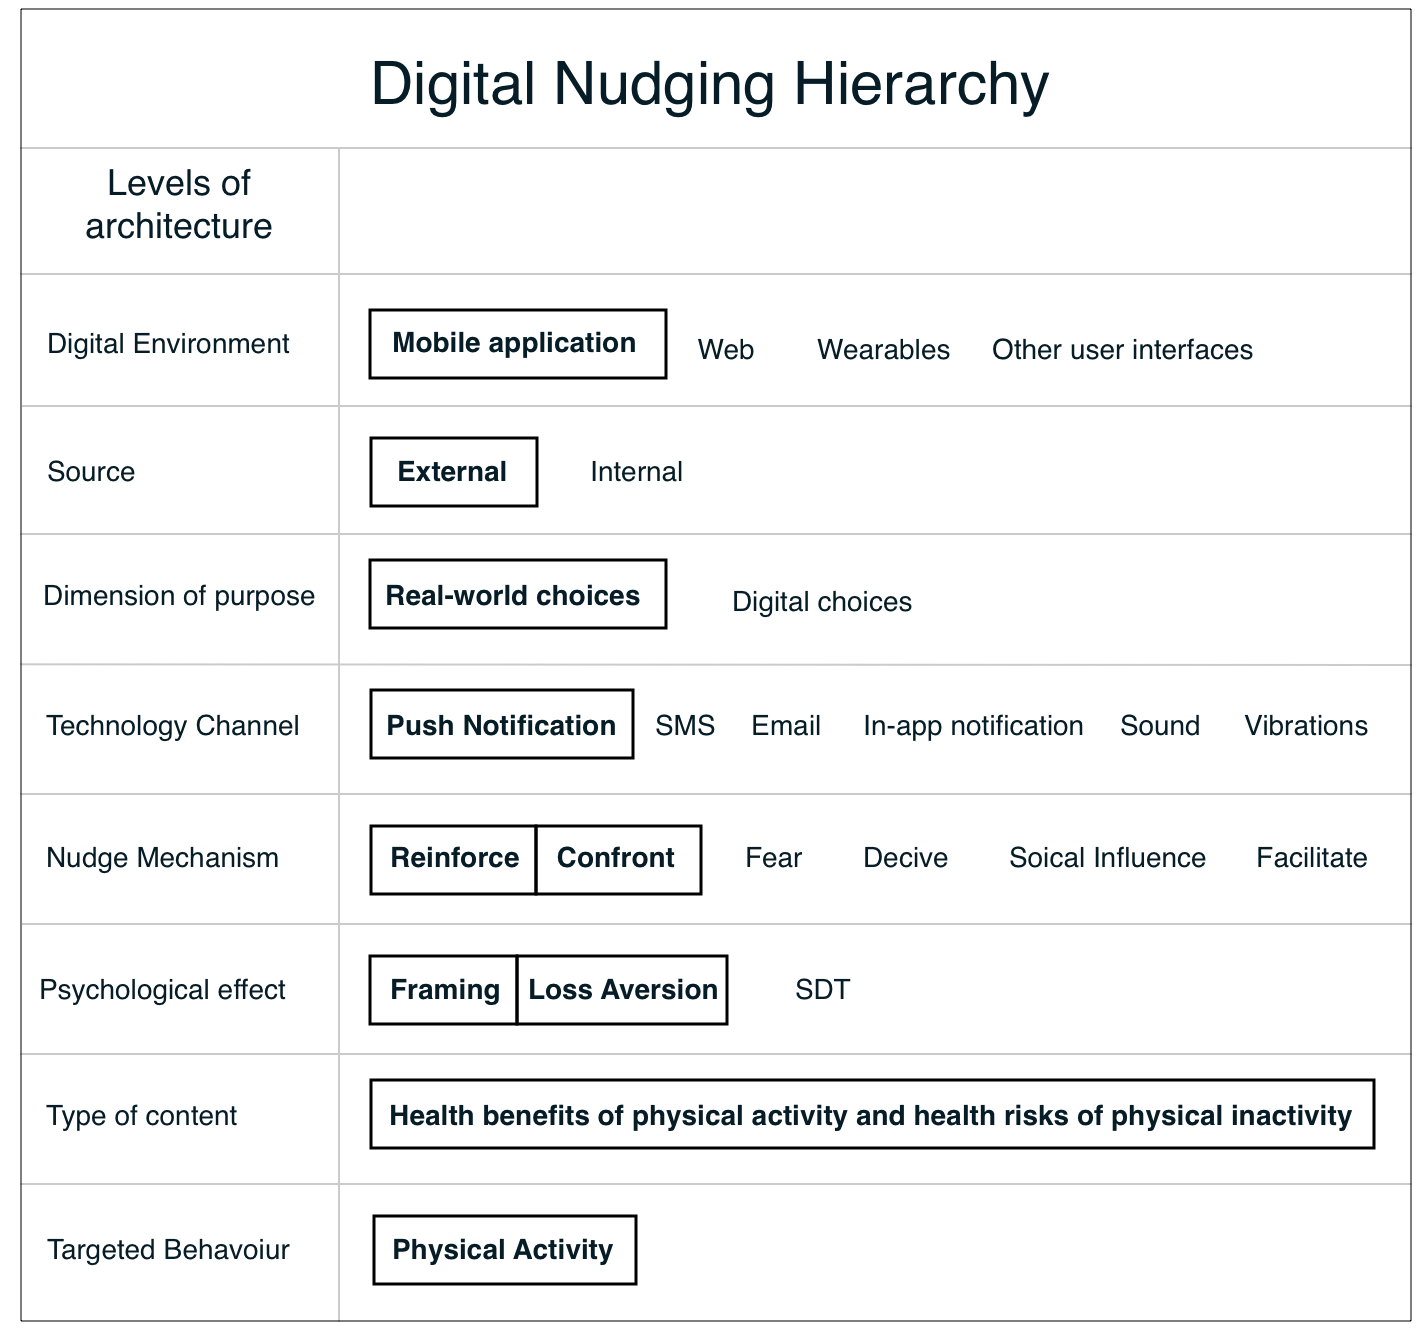
\includegraphics[width=1\textwidth]{Artboard6.png}
\caption{A delineation of the scope can be illustrated by a pseudo hierarchy that distinguish and sort the terms}
\end{figure}
\bigbreak
\bigbreak


\begin{table}[ht]
\begin{tabular}{|l|l|}
\hline
\multicolumn{2}{|l|}{\textbf{Phase 1}} \\ \hline
R1 &  \\ \hline
R2 &  \\ \hline
R3 &  \\ \hline
R4 &  \\ \hline
R5 &  \\ \hline
\multicolumn{2}{|l|}{\textbf{Phase 2}} \\ \hline
R6 &  \\ \hline
R7 &  \\ \hline
R8 &  \\ \hline
\multicolumn{2}{|l|}{\textbf{Phase 3}} \\ \hline
R9 &  \\ \hline
R10 &  \\ \hline
\end{tabular}
\end{table}

\begin{comment}
%"Selve push meldingen (den som operativsystemet gir bruker, og lever på utsiden av appen); Her bruker vi Google Firebase for å kommunisere med telefonen. Den tar utgangspunkt i Device ID (telefonen) og pusher til Device ID eller IDer (om brukeren er registert med flere devicer). Dette oppfattes som selve push-meldingen. Det er vår serviceplattform som kommuniserer med Google Firebase (og CMSet du kjenner til er det som pusher informasjon inn til vår service plattform). Vår service plattform er forresten ren Microsoft Azure."
\end{comment}

\begin{comment}
%KODEN ER RIKTIG
% Please add the following required packages to your document preamble:
% \usepackage{multirow}
% \usepackage[normalem]{ulem}
% \useunder{\uline}{\ul}{}
\begin{table}[]
\begin{adjustwidth}{}{}
\begin{tabular}{|l|l|l|}
\hline
\multirow{5}{*}{\textbf{\begin{tabular}[c]{@{}l@{}}Phase 1: \\ Analyse\end{tabular}}} & \begin{tabular}[c]{@{}l@{}}R1: Definition of organizational\\ goals\end{tabular} & \begin{tabular}[c]{@{}l@{}}Help members achieve the \\ recommendations of physical \\ activity given by the authorities\end{tabular} \\ \cline{2-3} 
 & \begin{tabular}[c]{@{}l@{}}R2: Definition of desired user \\ behaviour\end{tabular} & \begin{tabular}[c]{@{}l@{}}Engaing in regular physical \\ activity\end{tabular} \\ \cline{2-3} 
 & R3: Analysis of user goals & \begin{tabular}[c]{@{}l@{}}User goals vary, but they share \\ the intention to be physical \\ active (at some level)\end{tabular} \\ \cline{2-3} 
 & \begin{tabular}[c]{@{}l@{}}R4: Analysis of user characteristics \\ and decision-making process\end{tabular} &  \\ \cline{2-3} 
 & \begin{tabular}[c]{@{}l@{}}R5: Definition of technology \\ channel\end{tabular} & \begin{tabular}[c]{@{}l@{}}Push notification integrated \\ in Sats app\end{tabular} \\ \hline
\multirow{3}{*}{\textbf{\begin{tabular}[c]{@{}l@{}}Phase 2: \\ Design\end{tabular}}} & R6: Selection of design principles & Framing effect \\ \cline{2-3} 
 & R7: Design of intervention & \begin{tabular}[c]{@{}l@{}}Users will receive different \\ digital nudges providing \\ them with health related \\ information\end{tabular} \\ \cline{2-3} 
 & \begin{tabular}[c]{@{}l@{}}R8: Identification and imitation of \\ successful interventions\end{tabular} & \begin{tabular}[c]{@{}l@{}}Developing persuasive \\ messages for physical \\ activity promotion...\end{tabular} \\ \hline
\multirow{2}{*}{\textbf{\begin{tabular}[c]{@{}l@{}}Phase 3: \\ Implementation \\ and Evaluation\end{tabular}}} & \begin{tabular}[c]{@{}l@{}}R9: Implementation and evaluation \\ of intervention effectiveness\end{tabular} & Qualitative evaluation through interviews \\ \cline{2-3} 
 & \begin{tabular}[c]{@{}l@{}}R10: Return to previous phases if \\ needed\end{tabular} & Not applicable \\ \hline
\end{tabular}
\caption{\label{tab:table-name}This table shows positive and negative statements related to gain and loss.}
\end{adjustwidth}{}{}
\end{table}
\end{comment}